\chapter{Decompositions of Edge Labels by decomposing Unary DFAs}
\label{ch:Analysis}
%% ==============================

As our goal is to represent general dynamic networks and temporal graphs as EPGs, one problem is the missing periodicity in general temporal and dynamic graphs. 

\begin{figure}[h]
	\begin{minipage}[t]{0.49\textwidth}
		\centering
		\begin{tikzpicture}[every edge quotes/.style = {auto, font=\footnotesize, sloped}]
			\begin{scope}[every node/.style={circle,fill}]
				\node (A) at (0,0) {};
				\node (B) at (0,2) {};
				\node (C) at (2,0) {};
				\node (D) at (2,2) {};
				\node (E) at (1,3) {};
			\end{scope}
			
			\draw (A) edge["101\dots"] (B)
			(B) edge["100\dots"] (C)
			(D) edge["001\dots"] (C)
			(A) edge["000\dots"] (C)
			(D) edge["111\dots"] (E)
			(B) edge["011\dots"] (D)
			(B) edge["101\dots"] (E);	
		\end{tikzpicture}
		
	\end{minipage}
	\begin{minipage}[t]{0.49\textwidth}
		\centering
		\begin{tikzpicture}[every edge quotes/.style = {auto, font=\footnotesize, sloped}]
			\begin{scope}[every node/.style={circle,fill}]
				\node (A) at (0,0) {};
				\node (B) at (0,2) {};
				\node (C) at (2,0) {};
				\node (D) at (2,2) {};
				\node (E) at (1,3) {};
			\end{scope}
			
			\draw (A) edge["101"] (B)
			(B) edge["100"] (C)
			(D) edge["0010"] (C)
			(A) edge["0"] (C)
			(D) edge["110"] (E)
			(B) edge["01111"] (D)
			(B) edge["10"] (E);
		\end{tikzpicture}
	\end{minipage}
	\caption{TODO}
\end{figure}

To transform a temporal graph, a shortest possible string $w'$ which is equal to the original label at every time step $\forall t \geq 0, \tau(e)[t] = w'[t]$ has to be found. This $w'$ can itself be composed by combining different factors $w_1,w_2,\dots,w_n$. Initially, we start with a temporal graph where all edge labels $\tau(e)$ have fixed length and there are no periods present. To find and analyze such periods in the given labels, the algorithm from \cite{DBLP:journals/corr/abs-2107-04683} is used and adapted to our problem. To apply the algorithm which is defined for automata, a label $ w \in \{0,1\}^*$ is interpreted as an unary automata. In the label either the $0s$ or the $1s$ symbols are used to represent final states $Q_f$. The algorithm from \cite{DBLP:journals/corr/abs-2107-04683} can be simplified due to the fact that we only represent unary automata with \textbf{$|\Sigma| = 1$} and therefore only have a single transition from each state, basically forming a simple circle of all possible states. Using the fact that our alphabet is of size one, we only need to follow a single transition and furthermore, we only need to check multiples of the chosen period. This means that for a period length of $i$ we only have to check $i$ states on the circle being in the same state.

\section{Decompositions of DFAs}
\label{sec:decomposition-unary-dfas}

\begin{figure}[h]
	\begin{minipage}[t]{0.29\textwidth}
		\centering
		Label $w=1001$
	\end{minipage}
	\begin{minipage}[t]{0.69\textwidth}
		\centering
		\begin{tikzpicture}[shorten >=1pt,node distance=2cm,on grid,auto] 
			\node[state,initial,accepting] (q_0)   {$q_0$}; 
			\node[state] (q_1) [right=of q_0] {$q_1$}; 
			\node[state] (q_2) [right=of q_1] {$q_2$}; 
			\node[state,accepting](q_3) [right=of q_2] {$q_3$};
			\path[->] 
			(q_0) edge  node {} (q_1)
			(q_1) edge  node {} (q_2)
			(q_2) edge  node {} (q_3)
			(q_3) edge[bend right, above]  node {} (q_0);
		\end{tikzpicture}
		\begin{tikzpicture}[shorten >=1pt,node distance=2cm,on grid,auto] 
			\node[state,initial] (q_0)   {$q_0$}; 
			\node[state,accepting] (q_1) [right=of q_0] {$q_1$}; 
			\node[state,accepting] (q_2) [right=of q_1] {$q_2$}; 
			\node[state](q_3) [right=of q_2] {$q_3$};
			\path[->] 
			(q_0) edge  node {} (q_1)
			(q_1) edge  node {} (q_2)
			(q_2) edge  node {} (q_3)
			(q_3) edge[bend right, above]  node {} (q_0);
		\end{tikzpicture}
	\end{minipage}
	\caption{Equivalence of binary strings and unary permutation \DFAs}
\end{figure}

A DFA $\mathcal{A}$ is composite if its language $L(\mathcal{A})$ can be decomposed into an intersection $\cup^k_{i=1} L(\mathcal{A}_i)$ of languages of smaller DFAs. Otherwise, $\mathcal{A}$ is prime. This notion of \textit{primality} was introduced by Kupferman and Mosheiff in \cite{prime-languages}, and they proved that we can decide whether a DFA is composite in ExpSpace and later in \cite{unara-prime-languages}, the decomposition question for unary DFAs was proven to be in \LogSpace. In the paper~\cite{DBLP:journals/corr/abs-2107-04683} by Jecker, Mazzocchi and Wolf, they provided a \LogSpace algorithm for commutative permutation DFAs, if the alphabet size is fixed, which also puts the bounded $k$-composite question for unary DFAs in the \LogSpace complexity class, see \ref{tab:dfa-decomp-complexity} for further reference. The decomposition of unary \DFAs are usually characterized by means of clean quotients. Let  $A = \lbrace\Sigma, Q, q_I , \sigma, F\rbrace$ be a unary-DFA. A clean quotient $A_d$ of $A$ is a DFA obtained by folding its cycle of length $l$ to a cycle of length $d$, for some strict divisor $d$ of $l$. Formally, $A_d$ is induced by the equivalence relation $\sim_d$ defined by

\[ q_i \sim_d q_j ~\text{if and only if}~i \equiv j ~mod~ d \]

Since $\sim_d$ is coherent with $\sigma$, and therefore $L(A) \subseteq L(A_d)$.

\begin{figure}[h]
	\begin{minipage}[t]{\textwidth}
		\centering
		\begin{tikzpicture}[shorten >=1pt,node distance=2cm,on grid,auto] 
			\node[state,initial] (q_0)   {$q_0$}; 
			\node[state,accepting] (q_1) [ right=of q_0] {$q_1$}; 
			\node[state] (q_2) [ right=of q_1] {$q_2$}; 
			\node[state,accepting] (q_3) [ right=of q_2] {$q_3$};
			\node[state](q_4) [ right=of q_3] {$q_4$};
			\path[->] 
			(q_0) edge  node {} (q_1)
			(q_1) edge  node {} (q_2)
			(q_2) edge  node {} (q_3)
			(q_3) edge  node {} (q_4)
			(q_4) edge[bend right, above]  node {} (q_0);
		\end{tikzpicture}		
	\end{minipage}
	\begin{minipage}[b]{0.49\textwidth}
		\centering
		\begin{tikzpicture}[shorten >=1pt,node distance=2cm,on grid,auto] 
		\node[state,initial,accepting] (q_0)   {$q_0$}; 
		\node[state,accepting] (q_1) [right=of q_0] {$q_1$}; 
		\node[state](q_2) [right=of q_1] {$q_2$};
		\path[->] 
		(q_0) edge  node {} (q_1)
		(q_1) edge  node {} (q_2)
		(q_2) edge[bend right, above]  node {} (q_0);

\end{tikzpicture}
	\end{minipage}
	\begin{minipage}[b]{0.49\textwidth}
		\centering
		\begin{tikzpicture}[shorten >=1pt,node distance=2cm,on grid,auto] 
		\node[state,initial] (q_0)   {$q_0$}; 
		\node[state,accepting] (q_1) [right=of q_0] {$q_1$}; 
		\path[->] 
		(q_0) edge  node {} (q_1)
		(q_1) edge[bend right, above]  node {} (q_0);
		\end{tikzpicture}
	\end{minipage}
	\caption{The DFA $A$ and its clean quotients $A_1$ and $A_2$}
\end{figure}

TODO: Explain example

\subsection{Decomposing using maximal divisors}
Usually the algorithms and proofs are considering unary \DFAs consisting of a chain leading into a cycle of states. Since we obtain our \DFAs by transforming from a periodic label, we only have \DFAs with empty chains, therefore only considering unary permutation \DFA. This allows us to use a slightly simplified version of the Algorithm from \cite{DBLP:journals/corr/abs-2107-04683} as seen in Algorithm \ref{algo:composite} as we do not encounter unary automata with $\sigma(q, uv) \not = \sigma(q, vu)$. Additional we are not only interested in answering the yes/no question of the composite problem but we actually want to collect the factors and continue our computation.

\begin{algorithm}[H]
	\label{algo:composite}
	\DontPrintSemicolon
	\SetKwProg{Fn}{Function}{:}{}
	\Fn{getComposite($A = ⟨{a}, Q, qI , \sigma, F ⟩ $: unary DFA, integer k)}{
		FactorList $\gets \emptyset$\; 
		\ForEach{binaryString $\in \{0,1\}^{log|Q|}$ with $\leq k$ ones}{
			\If{isFactor($A$,binaryString)}{FactorList.add(binaryString)}
		}
		\KwRet FactorList\;
	}

	\Fn{isFactor($A = ⟨{a}, Q, qI , \sigma, F ⟩ $: unary DFA, binaryString)}{
		\ForEach{$q \in Q \setminus F$}{
			\If{not cover(A,q,binaryString)}{\KwRet false}
			\KwRet true
		}
	}
	
	\Fn{cover($A = ⟨{a}, Q, qI , \sigma, F ⟩ $: unary DFA, binaryString, $q \in Q \setminus F$)}{
		\ForEach{$i$ with wordCombination[i]=1}{
			$p_1 \gets i$'th prime divisor of $|Q|$\;
			\If{cover($A,q,\sigma(q,a^{|Q|/p_i})$)}{\KwRet true}
		}
		\KwRet false
	}
	
	\caption{LOGSPACE-algorithm solving the Decomp problem for unary DFAs and returning the factors.}
\end{algorithm}

TODO: explain algo and difference to original

TODO complexity

\subsection{Short Factors}

\subsection{Fourier Transform}

\section{Combining factors into a EPG label}

Now with the collection of periods, novel problems arises. How to combine the periods in the most optimal manner? What is the minimal number of periods needed to cover a given array? These and other questions where tried to answer both theoretically and empirically with some real world data.

\section{Modified Decomposition Problem}
\begin{figure}[h]
	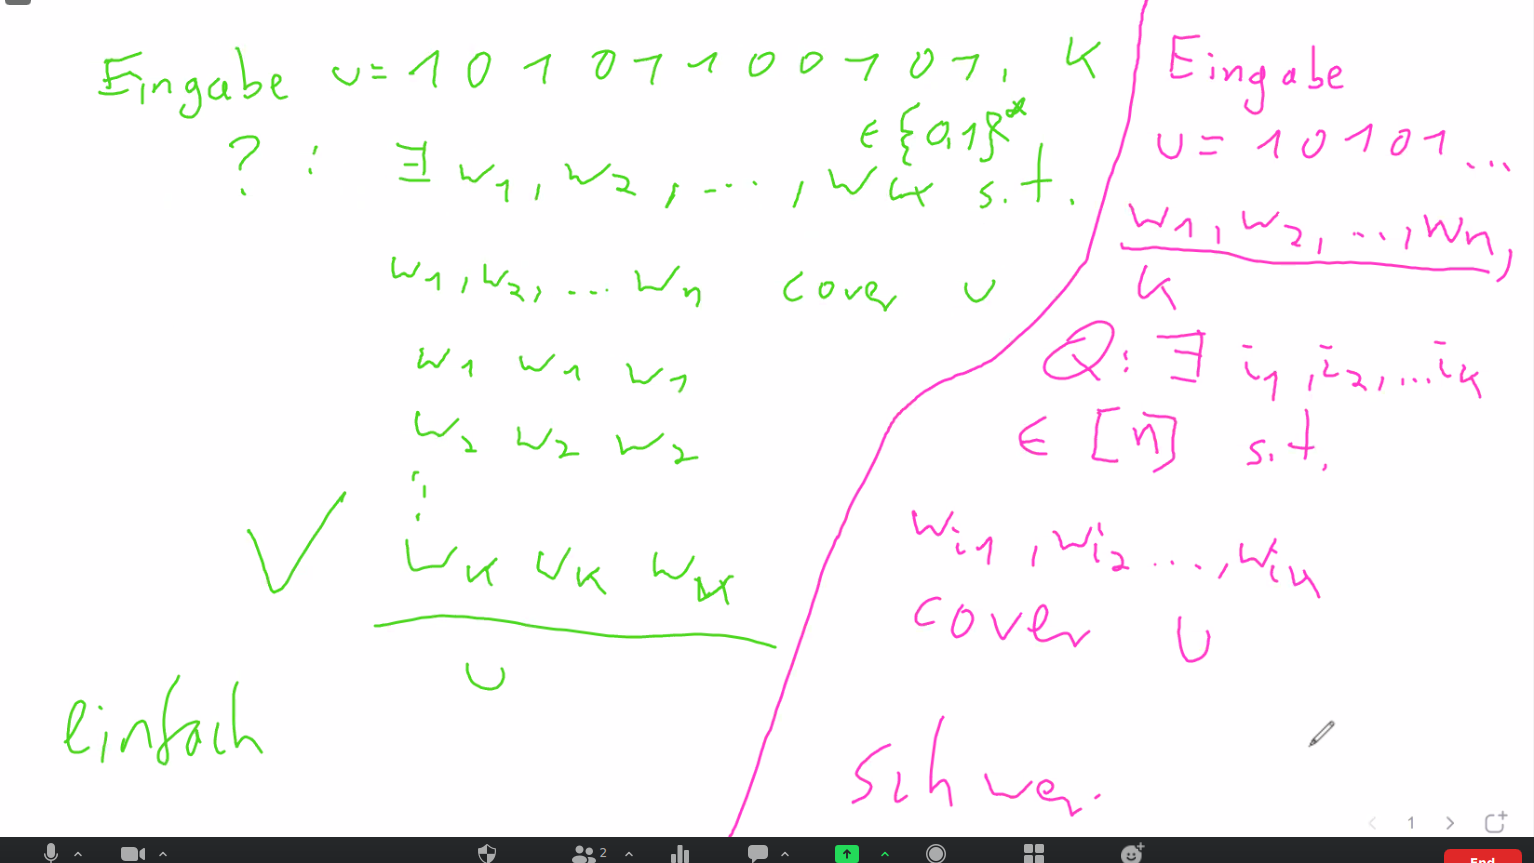
\includegraphics[width=\linewidth]{proof-sketches/Screenshot[2]-01.png}
\end{figure}

